% -*- latex -*-
\author{Adam Pilewski, \textbf{311382}}
\title{PGUI, Kamień milowy \\1}
\frenchspacing
\documentclass[a4paper,11pt]{article}

\usepackage[T1]{polski}
\usepackage[utf8]{inputenc}
\usepackage{pdfpages}
\usepackage{graphicx}
\usepackage{hyperref}
\hypersetup{
    colorlinks=true,
    linkcolor=blue,
    filecolor=magenta,      
    urlcolor=cyan,
    pdftitle={Overleaf Example},
    pdfpagemode=FullScreen,
    }

\setlength{\parindent}{0pt}
\setlength{\parskip}{\medskipamount}
\raggedbottom


\addtolength{\oddsidemargin}{-.999in}
\addtolength{\evensidemargin}{-.999in}
\addtolength{\textwidth}{2.2in}

\addtolength{\topmargin}{-.999in}
\addtolength{\textheight}{2.2in}

\begin{document}
\maketitle

\section{Analiza i wymagania}
\subsection{MoSCoW}


\begin{enumerate}
    \item MUST
    \begin{enumerate}
        \item 1sbeb
        \item 1sbeb
        \item 1sbeb
        \item 1sbeb
        \item 1sbeb
    \end{enumerate}
    \item SHOULD
    \begin{enumerate}
        \item Diagramy UML
        \item Figma
    \end{enumerate}
    \item COULD
    \begin{enumerate}
        \item 1sbeb
        \item 1sbeb
        \item 1sbeb
        \item 1sbeb
        \item 1sbeb
    \end{enumerate}
    \item WON'T
    \begin{enumerate}
        \item 1sbeb
        \item 1sbeb
        \item 1sbeb
        \item 1sbeb
        \item 1sbeb
    \end{enumerate}
\end{enumerate}
\section{UML}
\section{Figma}
\href{https://www.figma.com/file/fKp84G0oZXkCUW8J8Bf94M/PGUI-Panel-Sprzedawcy?node-id=303%3A40&t=JpyKh5oAmRAebYLE-0}{link do Figmy}
\section{Projekt implementacji}
\subsection{Biblioteki}
\begin{enumerate}
    \item Przechowywanie stanu
    \begin{enumerate}
        \item react-redux
        \item redux-persist
    \end{enumerate}
    \item CSS
    \begin{enumerate}
        \item tailwindcss
        \item clsx
    \end{enumerate}
    \item Nawigacja
    \begin{enumerate}
        \item react-router-dom
    \end{enumerate}
    \item Wykresy
    \begin{enumerate}
        \item recharts
    \end{enumerate}
\end{enumerate}
\subsection{Przechowywanie stanu}
\subsection{Szkielet implementacji}
\url{https://github.com/adas77/panel} \\
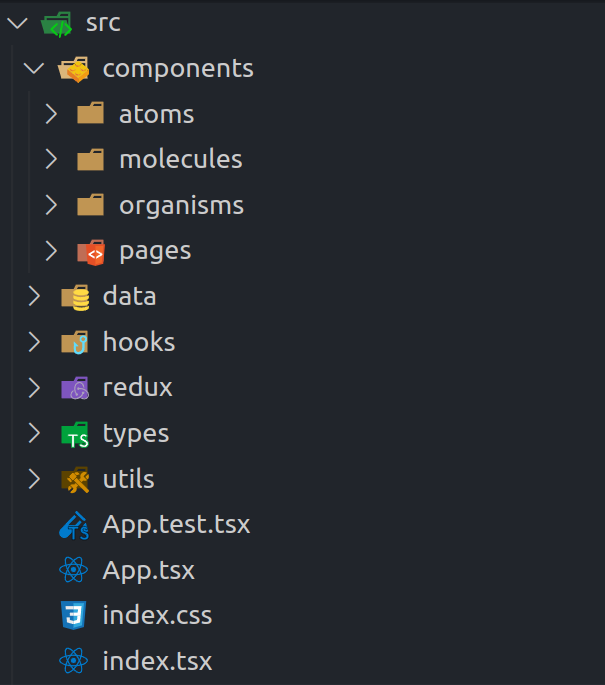
\includegraphics[scale=0.5]{src/s.png}

% \includepdf[pages=-]{src/}
% \includegraphics[scale=0.5]{src/}

\end{document}